\documentclass[titlepage,letterpaper,final,12pt]{scrartcl}

\usepackage[total={6.0in,8.75in},top=1.2in,left=1.35in]{geometry}

% this lets us avoid the scrartcl/hyperref conflict...
%\let\ifvtex\relax

\usepackage{verbatim}
\usepackage{empheq}
\usepackage[dvipsnames]{xcolor}
\usepackage{animate}
\usepackage{graphicx}
\usepackage{fancyvrb}

% hyperref should be the last package we load
\usepackage[pdftex,
colorlinks=true,
plainpages=false, % only if colorlinks=true
linkcolor=blue,   % only if colorlinks=true
citecolor=blue,   % only if colorlinks=true
urlcolor=blue     % only if colorlinks=true
]{hyperref}

\pdfinfo{
/Title (Numerical modelling of ice sheets, streams, and shelves)
/Author (Ed Bueler)
/Subject (numerical modelling of glaciers, ice sheets, and ice shelves)
/Keywords (numerical modelling, numerical analysis, glacier, ice sheet, ice shelf, shallow models of ice flow)
}

\newcommand{\ddt}[1]{\ensuremath{\frac{\partial #1}{\partial t}}}
\newcommand{\ddx}[1]{\ensuremath{\frac{\partial #1}{\partial x}}}
\newcommand{\ddy}[1]{\ensuremath{\frac{\partial #1}{\partial y}}}
\newcommand{\pp}[2]{\ensuremath{\frac{\partial #1}{\partial #2}}}
\renewcommand{\t}[1]{\texttt{#1}}
\newcommand{\Matlab}{\textsc{Matlab}\xspace}
\newcommand{\bq}{\mathbf{q}}
\newcommand{\bU}{\mathbf{U}}
\newcommand{\eps}{\epsilon}
\newcommand{\grad}{\nabla}
\newcommand{\Div}{\nabla\cdot}
\newcommand{\devstress}{\tau}

\newcommand{\mmess}[1]{\vspace{-0.1in}\begin{center}
\fbox{\url{http://www.dms.uaf.edu/~bueler/mccarthy/mfiles/#1.m}}
\end{center}}

\newcommand{\minput}[1]{
\bigskip
\begin{quote}
\bigskip
\VerbatimInput[frame=single,framesep=3mm,label=\fbox{\normalsize \textsl{\,#1.m\,}},fontfamily=courier,fontsize=\scriptsize]{../mfiles/#1.slim.m}
\bigskip
\end{quote}
}

%\onefigsize{name}{caption}{width}
\newcommand{\onefigsize}[3]{
\begin{figure}[ht]
\centering
\includegraphics[width=#3,keepaspectratio=true]{#1}
\caption{#2}
\label{fig:#1}
\end{figure}}

%\onefig{name}{caption}
\newcommand{\onefig}[2]{\onefigsize{#1}{#2}{3.0in}}

%\twofigsizes{left-name}{right-name}{caption}{left-width}{right-width}
\newcommand{\twofigsizes}[5]{
\begin{figure}[ht]
\centering
\includegraphics[width=#4,keepaspectratio=true]{#1} \quad
\includegraphics[width=#5,keepaspectratio=true]{#2}
\caption{#3}
\label{fig:#1}
\end{figure}}

%\twofig{left-name}{right-name}{caption}
\newcommand{\twofig}[3]{\twofigsizes{#1}{#2}{#3}{2.5in}{2.5in}}



\begin{document}
\graphicspath{{../photos/}{../pdffigs/}}


\begin{titlepage}

  \begin{center}
    {\Large\usekomafont{title} Numerical modelling \\ of ice sheets, streams, and shelves}
    \vspace{0.5cm}

    {\large Ed Bueler}
    \vspace{1cm}

    September 2012

    \vfill
    
    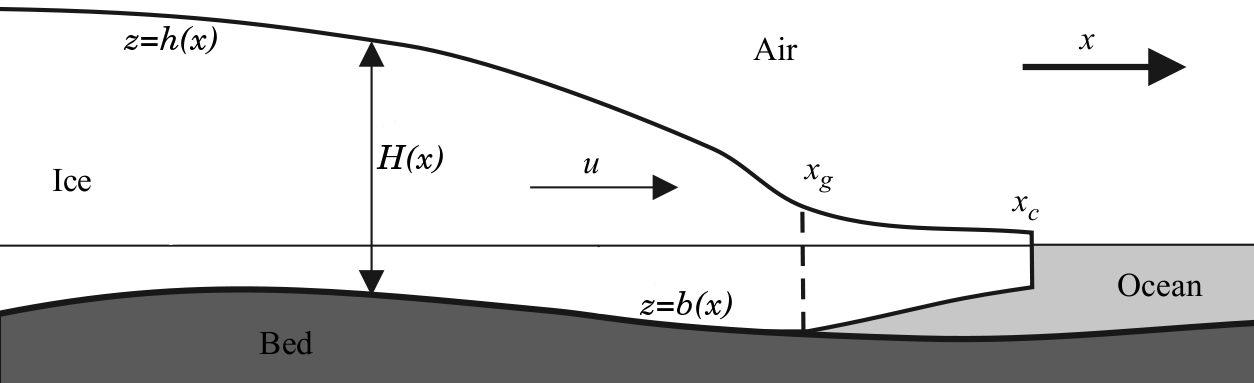
\includegraphics[width=6.0in]{flowline}
  
    \scriptsize \emph{Illustrates the notation used in this chapter.  Figure modified from \cite{SchoofMarine1}.} \normalsize
    
    \vspace{2.0in}
  \end{center}
\end{titlepage}

\clearpage\newpage

\setcounter{section}{1}
\subsection{Introduction}

Numerical models can, if well-constructed, actually help you, the reader, understand the behavior of particular glaciers, ice sheets, and ice shelves.  Their most common use may be to help you ask: When I put together my incomplete understanding of these processes into a mathematical model, does the combination behave as I expect?  Or why does it mis-behave?  Though numerical models rarely generate new theoretical understandings---a human brain seems to be needed to get new insights from observations!---they can demonstrate flaws in the understanding of glacier processes, or in how processes combine to give behavior.

Numerical models should be built with care.  The worst outcome is to have a researcher spend time explaining, through physical argumentation and using observational evidence, some model behavior that is simply an artifact of poor computer programming or numerical analysis.  The reader of this chapter may be surprised that the continuum model, and not the code, seems to be our focus much of the time.  This is because our intention to approximate the continuum model requires that we \emph{analyze} the numerical implementation to check that it matches the intent.  Such analysis is via an understanding of the continuum model and its solutions.  All numerical codes produce numbers of some kind, and many pretty pictures!  We want numbers and pictures that actually come from our continuum model.

This chapter has a limited scope
  \begin{quote}\emph{we focus on approximating ice flow}\end{quote}
and a constructive approach
  \begin{quote}\emph{we provide example numerical codes that actually work.}\end{quote}

Within our scope are the shallow ice approximation (SIA) in two horizontal dimensions (2D), the shallow shelf approximation (SSA) in 1D, and the mass continuity and surface kinematical equations.  We briefly describe the Stokes model, but we do not address its numerical solution.  The numerical ideas include finite difference schemes, solving algebraic systems from stress balances, and the verification of numerical codes.

Our notation is generally common to the glaciological literature; see Table \ref{tab:notation}.  Coordinates are $t,x,y,z$, with $z$ perpendicular to the geoid and positive-upward.  If the coordinates appear as subscripts then these denote partial derivatives: $u_x = \partial u/\partial x$.  Tensor notation uses subscripts from the list $\{1,2,3,i,j\}$, so that, for example, $\tau_{ij}$ is a generic entry, and $\tau_{13}$ a particular entry, of the deviatoric stress tensor.

This chapter is based on sixteen Matlab (or Octave) codes, each about one-half page.  Six are printed in this text.  They are all distributed in \texttt{.zip} form at\footnote{And on a USB memory stick at Karthaus.}
\begin{quote}
\fbox{\url{http://www.dms.uaf.edu/~bueler/karthaus/}}
\end{quote}
\noindent When displayed in these notes these codes have all their comments stripped for compactness and clarity, while the electronic versions have generous comments and help.

\subsubsection*{Ice flow equations}  My first goal in these notes is to get to an equation for which I can say:
\begin{center}
\emph{numerically solve this equation, and you've got a usable model for an ice sheet.}
\end{center}
Note that a ``usable'' model is \emph{understood} more than it is \emph{correct}.  To get to my goal I will quickly recall the continuum mechanical equations of ice flow.  

\begin{table}
\caption{Notation used in this chapter.}
\label{tab:notation}
\begin{tabular}{cll}
variable  & description & SI units \\ 
\hline
$A$ & $A=A(T)=$ ice softness in the Glen flow law & $\text{Pa}^{-3}\,\text{s}^{-1}$ \\
$B$ & ice hardness; $B=A^{-1/n}$ & $\text{Pa}\,\text{s}^{1/3}$ \\
$b$ & bedrock elevation & m \\
$\nabla$ & (spatial) gradient & m$^{-1}$ \\
$\nabla\cdot$ & (spatial) divergence & m$^{-1}$ \\
$\nabla^2$ & (spatial) Laplacian: $\nabla^2 f = \nabla\cdot(\nabla f)$ & m$^{-2}$ \\
$g$ & gravity & m s$^{-2}$ \\
$H$ & ice thickness & m \\
$h$ & ice surface elevation & m \\
$M$ & climatic mass balance & m s$^{-1}$ \\
$n$ & exponent in Glen flow law & \\
$\nu$ & viscosity & Pa s \\
$p$ & pressure & Pa \\
$\bq$ & map-plane ice flux: $\bq = \int_{b}^{h} \mathbf{u}\,dx = \bar{\mathbf{u}} H$ & $\text{m}^2\,\text{s}^{-1}$ \\
$\rho$ & density of ice & kg m$^{-3}$ \\
$\rho_w$ & density of sea water & kg m$^{-3}$ \\
$T$ & temperature & K \\
$\tau$ & magnitude of $\tau_{ij}$: $2 \tau^2 = \sum_{ij} \tau_{ij}^2$ & Pa \\
$\tau_{ij}$ & deviatoric stress tensor & Pa \\
$Du_{ij}$ & strain rate tensor & s$^{-1}$ \\
$\mathbf{U}$ & $=(u,v)$ horizontal ice velocity & m s$^{-1}$ \\
$\mathbf{u}$ & $=(u,v,w)$ ice velocity & m s$^{-1}$ \\
\end{tabular}
\end{table}

Ice in glaciers is a fluid.  We describe the flow of fluids primarily by a \emph{velocity field} $\mathbf{u}(t,x,y,z)$.  If the ice fluid were either faster-moving than it actually is (e.g., because gravity was much stronger), and if it were linearly-viscous (with viscosity $\nu$) like liquid water, then it would be a ``typical'' fluid.  We would use the Navier-Stokes equations as the model:
\begin{align}
\nabla \cdot \mathbf{u} &= 0 &&\text{\emph{incompressibility}} \label{incompressible} \\
\rho \left(\mathbf{u}_t + \mathbf{u}\cdot\nabla \mathbf{u}\right) &= -\nabla p + \nu \nabla^2 \mathbf{u} + \rho \mathbf{g} &&\text{\emph{stress balance}} \label{navierstokes}
\end{align}
In Equation \eqref{navierstokes} the term in parentheses is an acceleration.  The right-hand side is the total stress, and the equation says ``$ma=F$'', i.e.~Newton's second law.

You say ``\emph{hmmm} \dots \emph{does not sound like glaciology to me!}''  Indeed, is numerical ice flow modeling a part of computational fluid dynamics?  Emphatically ``yes''.  It is a large scale fluid problem like atmosphere and ocean modelling in climate systems.

But it is a weird one!  Consider the topics which make ocean flow modelling exciting:
  \begin{center} turbulence \qquad convection \qquad  coriolis force  \qquad salinity \qquad chemistry
  \end{center}
None of this topic list is relevant to ice flow.  (So what could be interesting about the flow of slow, laminar, boring old ice?)

We observe that ice is a slow, shear-thinning fluid.  In terms of equations, ``slow'' implies that $\rho \left(\mathbf{u}_t + \mathbf{u}\cdot\nabla \mathbf{u}\right) \approx 0$, which is to say that the forces of inertia are negligible.  Glaciers also have shear-thinning flow---a specific ``non-Newtonian'' behavior in which larger strain rate implies smaller viscosity.  Thus the viscosity $\nu$ in \eqref{navierstokes} is not constant, and we replace it by a ``flow law'', the famous Glen law.

Thus the standard ``full'' model for isothermal flow is the set of Stokes equations:
\begin{align}
\nabla \cdot \mathbf{u} &= 0 &&\text{\emph{incompressibility}} \label{incompressibleagain} \\
0 &= - \nabla p + \nabla \cdot \tau_{ij} + \rho \mathbf{g} &&\text{\emph{stress balance}} \label{forcebalance} \\
Du_{ij} &= A \tau^2 \tau_{ij} &&\text{\emph{$n$=3 Glen flow law}} \label{flowlaw}
\end{align}
In the flow law, the deviatoric stress tensor $\tau_{ij}$ and the strain rate tensor $Du_{ij}$ appear; previous lectures cover these.  Here we merely note that each tensor has trace zero, and also that $2\,Du_{ij} = (u_i)_{x_j}+(u_j)_{x_i}$.

The Stokes equations do not contain a time derivative of the unknowns (i.e.~$\mathbf{u}$ and the stresses).  Therefore geometry, boundary stresses, and ice softness together determine the velocity and stress fields instantaneously.  In fact, ice flow simulation codes have no memory of momentum or velocity.  Velocity is a ``diagnostic'' output which is not needed for restarting a simulation.


\subsubsection*{Slab-on-a-slope}  Consider now the $x,z$-plane flow case of equations \eqref{incompressibleagain}, \eqref{forcebalance}, and \eqref{flowlaw}.  ``Plane flow'' means that $v=0$ and all derivatives with respect to $y$ are zero:
\begin{empheq}[]{align}
u_x + w_z &= 0 &&\text{\emph{incompressibility}} \label{incompressiblexz} \\
p_x &= \tau_{11,x} + \tau_{13,z} &&\text{\emph{stress balance} ($x$)} \label{stokespx} \\
p_z &= \tau_{13,x} - \tau_{11,z} - \rho g &&\text{\emph{stress balance} ($z$)} \label{stokespz} \\
u_x &= A \tau^2 \tau_{11} &&\text{\emph{flow law} (diagonal)}  \label{forceflowx} \\
u_z + w _x &= 2 A \tau^2 \tau_{13} &&\text{\emph{flow law} (off-diagonal)} \label{forceflowz}
\end{empheq}
(Recall $x,z$ subscripts denote partial derivatives.)  Note that $\tau_{13}$ is a ``vertical'' shear stress while $\tau_{11}$ and $\tau_{33}=-\tau_{11}$ are deviatoric longitudinal stresses.  Also $\tau = (\tau_{11}^2+\tau_{13}^2)^{1/2}$ in this case.

This is a system of five nonlinear equations in five unknowns ($u,w,p,\tau_{11},\tau_{13}$).  This may be complicated enough to make you, like many before, pause before jumping in to a numerical solution method.  Can we handle a simplified situation?  Our first example is both a case in which we actually solve the Stokes equations, and a motivation for the shallow model which follows.  The example is a slab-on-a-slope, that is, we suppose there is no variation in $x$.

We will use rotated coordinates in this first example (and not elsewhere in these notes).  Consider the two-dimensional axes ($x$,$z$) shown in Figure \ref{fig:slab}, which are rotated downward at angle $\alpha>0$ so that the gravity vector has components $\mathbf{g} = (g \sin\alpha,- g \cos \alpha)$.  Equations \eqref{stokespx}, \eqref{stokespz}, in rotated coordinates, are
\begin{align}
p_x &= \tau_{11,x} + \tau_{13,z} + \rho g \sin\alpha, \label{stokespxrot} \\
p_z &= \tau_{13,x} - \tau_{11,z} - \rho g \cos\alpha. \label{stokespzrot}
\end{align}

\onefig{slab}{Configuration of slab-on-a-slope flow calculation.}

Because there is no variation with $x$, the whole set of Stokes equations \eqref{incompressiblexz}, \eqref{forceflowx}, \eqref{forceflowz}, \eqref{stokespxrot}, \eqref{stokespzrot} simplifies greatly:
\begin{align*}
w_z &= 0 &   0 &= \tau_{11} \\
\tau_{13,z} &= - \rho g \sin\theta &   u_z &= 2 A \tau^2 \tau_{13} \\
p_z &= - \rho g \cos\theta
\end{align*}
We apply boundary conditions for these functions of $z$:
	$$w(0)=0, \qquad p(H)=0, \qquad u(0)=u_0.$$
The basal velocity $u_0$ will remain undetermined for now.  By integrating vertically, we get $w=0$, $p = \rho g \cos\theta (H-z)$, and a linear formula for the shear stress,
	$$\tau_{13} = \rho g \sin\theta (H-z).$$
Note that $H-z$ is the depth within the ice.  Finally we also get a formula for the horizontal velocity,
\begin{equation}
u = u_0 + 2 A (\rho g \sin\theta)^3 \int_0^z (H-z')^3\,dz' = u_0 + \frac{1}{2} A (\rho g \sin\theta)^3  \left(H^4 - (H-z)^4\right) \label{uslab}
\end{equation}

Do we believe these equation \eqref{uslab}?  Figure \ref{fig:slabvel} compares its velocity to observations of a mountain glacier.  We have done a credible job of capturing deformation flow velocity, though we do not yet have a model for the sliding velocity $u_0$.  

\twofigsizes{slabvel}{athabasca_deform}{Left:  Velocity from the slab-on-a-slope calculation.  Right:  Velocity in a mountain glacier (Athabasca Glacier, Canada), from inclinometry \cite{SavagePaterson}.}{2.2in}{2.0in}

Now that we have calculated the velocity $u$, so what?  The equations so far do not address the change in shape of the glacier or ice sheet.  For this we need another equation, the \emph{mass continuity} equation.  To explain it, suppose our slab has variable thickness $H=H(t,x)$ and define the vertical average of velocity:
	$$\bar u(x,t) = \frac{1}{H}\int_0^{H} u(t,x,z)\,dz.$$
The product $\bar u\, H$ is the rate of flow input into the side of the area in Figure \ref{fig:slabmasscontfig}.

Now, how does the ice area $A$ in the figure change?\footnote{In three-dimensions it would be ``How does the ice volume change?''}  We compute
	$$\frac{dA}{dt} = \int_{x_1}^{x_2} M(x)\,dx + \bar u_1 H_1 - \bar u_2 H_2$$
If the width $dx=x_2-x_1$ is small then $A\approx dx\, H$.  So we divide by $dx$ and get
\begin{equation}
H_t = M - \left(\bar u H\right)_x \label{masscont1D}
\end{equation}
This mass continuity equation describes the change in the ice thickness in terms of surface mass balance and also the ice velocity.  This is the most common ``use'' of the velocity in ice flow simulations.

\onefigsize{slabmasscontfig}{The mass continuity equation \eqref{masscont1D} follows from considering the changing area $A$ of ice (i.e.~in a planar flow).  Ice can be added at the top by mass balance $M$.  A difference of flow into left and right sides also changes $A$.}{2.5in}


\subsection{Shallow ice sheets}

Our slab-on-a-slope example gives us a rough explanation of the shallow ice approximation (SIA), which is a model we will use more generally.  From the slab-on-slope velocity formula \eqref{uslab} in the $u_0=0$ case (non-sliding case) we get
\begin{equation}
\bar u H = \int_0^H \frac{1}{2} A (\rho g \sin\theta)^3  \left(H^4 - (H-z)^4\right)\,dz = \frac{2}{5} A (\rho g \sin\theta)^3 H^5. \label{siaubar}
\end{equation}
Note that $\sin \theta \approx \tan\theta = - h_x$.  Combining these with mass continuity \eqref{masscont1D} gives
\begin{equation}
  H_t = M + \left(\frac{2}{5} (\rho g)^3 A H^5 |h_x|^2 h_x\right)_x. \label{sia1D}
\end{equation}

Equation \eqref{sia1D} is the main SIA equation.  It determines the evolution of ice sheets in terms of mass balance, ice softness, and bed elevation; note $h=H+b$.  Additional arguments are needed to actually show that the SIA is ``general purpose'' and not special to a simple slab.  Such arguments derive the SIA model from the Stokes equations, under the assumption that slopes and the depth-to-width ratio are small; see Notes and References.

We will numerically solve the SIA equation in section \ref{sec:numericalsia}.  First we seek to understand it better, and we will state it in two horizontal dimensions.

\subsubsection*{Understanding the shallow ice approx (SIA)}  Ice sheets have four outstanding properties as fluids.  They are (\emph{i}) slow, (\emph{ii}) shallow,  (\emph{iii}) non-Newtonian, and (\emph{iv}) they sometimes experience contact slip.  The first ice flow model we consider is the non-sliding, isothermal shallow ice approximation or ``SIA'' for short.  It applies to small depth-to-width ratio (``shallow'') grounded ice sheets on not-too-rough bed topography, whose flow is not dominated by sliding at the base.

Regarding ``shallow'', Figure \ref{fig:green_transect} shows a no-vertical-exaggeration version cross section of Greenland at $71^\circ$, as well as the standard vertically-exaggerated version which is far more familiar in the glaciological literature.  Remember that ice sheets are actually thin.

\onefig{green_transect}{A vertically-exaggerated cross section of the Greenland ice sheet ($71^\circ$ N) is shown by the vertical axis labels and the green and blue curves.  The version without such exaggeration is in red.}

The SIA uses the formulas from slab-on-a-slope, generalized to two horizontal dimensions.  Let $\mathbf{U} = (u,v)$ be the vector horizontal velocity.  The SIA uses a shear stress approximation
	$$(\tau_{13},\tau_{23}) \approx - \rho g (h-z) \nabla h.$$
From Equation \eqref{flowlaw}, and further approximation of the shear strain rates in planes parallel to the geoid, we get a formula for a strain rate,
\begin{equation*}
\mathbf{U}_z \approx 2 A |(\tau_{13},\tau_{23})|^{n-1} (\tau_{13},\tau_{23}) = - 2 A (\rho g)^n (h-z)^n |\nabla h|^{n-1} \nabla h.
\end{equation*}
By integrating vertically, in the non-sliding case, we get
\begin{equation}
\mathbf{U} = - \frac{2 A (\rho g)^n}{n+1} \left[H^{n+1} - (h-z)^{n+1}\right] |\nabla h|^{n-1} \nabla h.  \label{siavelocity}
\end{equation}

Mass continuity in two horizontal dimensions, which generalizes the 1D version \eqref{masscont1D}, also applies:
\begin{equation}
    H_t = M - \Div\left(\bar{\mathbf{U}} H\right)  \label{masscont}
\end{equation}
Combining Equations \eqref{siavelocity} and \eqref{masscont} and defining a positive constant $\Gamma = 2 A (\rho g)^n / (n+2)$, we get an equation for the rate of thickness change in terms of mass balance $M$, thickness, and surface slope $\grad h$:
\begin{equation}
H_t = M + \Div \left(\Gamma H^{n+2} |\grad h|^{n-1} \grad h \right) \label{sia}
\end{equation}

Fulfilling an earlier promise, if we just solve \eqref{sia} numerically then we get a usable model for the Barnes ice cap in Canada, see for example \cite{Mahaffy}.  The Barnes ice cap is a particularly simple, but real, ice sheet on a very flat bed.

\subsubsection*{Analogy with the heat equation}  An obligatory step toward understanding the SIA model is recognizing that Equation \eqref{sia} is analogous to the better-known heat equation.  All numerical methods for solving \eqref{sia} can be understood as modifications of well-known heat equation methods.

Recall first that the heat equation comes from simple empirical observations like Newton's law of cooling, the ordinary differential equation $dT/dt = -K (T-T_{\text{ambient}})$, 
where $T$ is the object's temperature and $K$ relates to its material and geometric properties (consider a cup of coffee \dots).  That is, Newton observed that the temperature of an object tends to decay exponentially to the temperature of its surroundings.  One way to derive the heat equation, a partial differential equation (PDE), is to argue that the segments of a rod also satisfy Newton's law of cooling.  Segment $j$ with temperature $T_j$ sees an ambient temperature which is the average of the segment's neighbors:
   $$\frac{dT_j}{dt} = -K \left(T_j - \frac{1}{2} (T_{j-1} + T_{j+1}) \right) = \frac{K}{2} \left(T_{j-1} - 2 T_j + T_{j+1}\right).$$
As segment lengths $\Delta x$ shrink to zero we see an approximation of the second derivative with respect to $x$ on the right because $K$ scales with $\Delta x^2$.  Thus the distributed temperature of a rod satisfies
\begin{equation}
  T_t = D T_{xx}. \label{heat1D}
\end{equation}
This is the one dimensional heat equation, at least when material properties are constant.  The constant $D$ is the ``diffusivity''.

The more complete 2D version of the heat equation describes the temperature $T(t,x,y)$ at position $x,y$ in an object and at time $t$.  Fourier's law, which is the formula $\mathbf{Q} = - k \grad T$ for heat flux, and conservation of energy replace the above ad hoc Newton's law of cooling argument.  If we allow an additional heat source $f$, conservation of energy says $\rho c T_t = f - \Div \mathbf{Q}$.  Combining these we get:
	$$\rho c T_t = f + \Div (k \grad T).$$
Here $\rho$ is density, $c$ is specific heat, and $k$ is conductivity.  Now define the ``diffusivity constant'' $D=k/(\rho c)$ and also $F = f/(\rho c)$.  Then the heat equation is
\begin{equation}
T_t = F + \Div (D\, \grad T). \label{heat}
\end{equation}
Figure \ref{fig:initialheat} shows a solution of the heat equation, where the initial condition is a localized ``hot spot''.  Solutions of the heat equation involve the spreading, in all directions, of any local heat maxima or minima, that is, diffusion.

\twofigsizes{initialheat}{finalheat}{A solution of the heat equation.  Left: Initial condition $T(0,x,y)$.   Right: Solution $T(t,x,y)$, computed numerically by \texttt{heat.m} below, at $t=0.02$.}{2.8in}{2.8in}

The SIA equation \eqref{sia} and the heat equation \eqref{heat} are each diffusive, time-evolving partial differential equations.  A side-by-side comparison is illuminating:
\begin{center}
\begin{tabular}{cc}
SIA:\, $H$ is ice thickness & \phantom{foo bar} heat: $T$ is temperature\phantom{foo bar}  \\
	\boxed{H_t = M + \Div \left({\color{red}\Gamma H^{n+2} |\grad h|^{n-1}}\, \grad h \right)}  &  \boxed{T_t = F + \Div (D\, \grad T)}
\end{tabular}
\end{center}
Notice that the number of derivatives (one time and two space derivatives) and the signs are the same in these equations.  Mass balance $M$ is analogous to the (scaled) heat source $F$.  

The analogy allows us to identify the diffusivity in the SIA:
	$$D = {\color{red}\Gamma H^{n+2} |\grad h|^{n-1}}.$$
The non-sliding shallow ice flow \emph{diffuses} the ice sheet.  When $\Gamma$ or $H$ or $|\grad h|$ are large, the diffusion acts more quickly.  This model (analogy) explains generally why the surfaces of ice sheets are quite smooth, at least if we ignor the non-fluid processes of crevassing and wind-driven snow.  There are, however, some issues with this analogy:  (\emph{i})  The thickness $H$ and surface elevation $h$ are not the same unless the bed is flat.  (\emph{ii})  The diffusivity $D$ depends on the solution $H$.  (\emph{iii}) The diffusivity $D$ goes to zero at margins, where $H\to 0$, and at divides and domes, where $|\grad h|\to 0$.


\subsection{Finite difference numerics} 

As already noted, numerical schemes for the heat equation are a good starting place for solving the SIA equation \eqref{sia} numerically, which is our goal.  Here we describe only finite difference schemes, with numerical alternatives left to the Notes and References.

Finite difference schemes replace derivatives in the differential equation by arithmetic.  The basic fact is \emph{Taylor's theorem}.  It says that for a smooth function $f(x)$,
	$$f(x+\Delta) = f(x) + f'(x) \Delta + \frac{1}{2} f''(x) \Delta^2 + \frac{1}{3!} f'''(x) \Delta^3 + \dots$$
You can replace ``$\Delta$'' by its multiples, for example:
\begin{align*}
f(x-\Delta) &= f(x) - f'(x) \Delta + \frac{1}{2} f''(x) \Delta^2 - \frac{1}{3!} f'''(x) \Delta^3 + \dots \\
f(x+2\Delta) &= f(x) + 2 f'(x) \Delta + 2 f''(x) \Delta^2 + \frac{4}{3} f'''(x) \Delta^3 + \dots
\end{align*}

The idea for constructing finite difference schemes is to combine expressions like those above to give approximations of derivatives.  Thereby one combines values of the unknown quantity from  locations on a grid.

Here we want partial derivative approximations, so we apply the Taylor's expansions one variable at a time.  For example with a general function $u=u(t,x)$ we can write these approximations:
\begin{align*}
u_t(t,x) &= \frac{u(t+\Delta t,x) - u(t,x)}{\Delta t} + O(\Delta t), \\
u_t(t,x) &= \frac{u(t+\Delta t,x) - u(t-\Delta t,x)}{2\Delta t} + O((\Delta t)^2), \\
u_x(t,x) &= \frac{u(t,x+\Delta x) - u(t,x-\Delta x)}{2\Delta x} + O((\Delta x)^2), \\
u_{xx}(t,x) &= \frac{u(t,x+\Delta x) - 2\, u(t,x) + u(t,x-\Delta x)}{\Delta x^2} + O((\Delta x)^2)
\end{align*}
Note that ``$+O(\Delta^2)$'' is better, in the sense that the approximation is closer, than ``$+O(\Delta)$'' if $\Delta$ is a small number.

\subsubsection*{Explicit scheme for the heat equation}  Now we can state the simplest ``explicit'' scheme for the 1D heat equation, namely PDE \eqref{heat1D} which is $T_t = D\, T_{xx}$.  In terms of the values of the solution $T(t,x)$ we would say
	$$\frac{T(t+\Delta t,x) - T(t,x)}{\Delta t} \approx D\,\frac{T(t,x+\Delta x) - 2\, T(t,x) + T(t,x-\Delta x)}{\Delta x^2}.$$
The finite difference scheme is not just an approximation of the PDE, but an actual method for computing numbers on a grid.  Let $(t_n,x_j)$ denote the time-space grid points.  Denote our approximation of the solution value on the grid $T(t_n,x_j)$ by $T_j^n$.\footnote{Evaluating the exact solution at a grid point gives a different value from the one we compute!}  Then the finite difference scheme is
	$$\frac{T_j^{n+1} - T_j^n}{\Delta t} = D\,\frac{T_{j+1}^n - 2\, T_j^n + T_{j-1}^n}{\Delta x^2}.$$
To get a simple, computable formula, let $\mu = D \Delta t / (\Delta x)^2$ and solve for $T_j^{n+1}$:
\begin{equation}
  T_j^{n+1} = \mu T_{j+1}^n + (1 - 2 \mu) T_j^n + \mu T_{j-1}^n \label{heat1Dfd}
\end{equation}
The scheme is ``explicit'' because we have been able to solve it for the next value we will compute.  Figure \ref{fig:expstencil} shows the ``stencil'' for scheme \eqref{heat1Dfd}: we use three values at the current time $t_n$ to update the one value at the next time $t_{n+1}$.

How accurate is \eqref{heat1Dfd}?  The above construction tells us that the difference between the scheme \eqref{heat1Dfd} and the PDE \eqref{heat1D} is $O(\Delta t,(\Delta x)^2)$.  This difference between equations goes to zero as we refine the grid in space and time (``consistency'').  With care about the smoothness of boundary conditions, and using mathematical facts about the heat equation itself, the theory of finite difference schemes shows that the difference between $T_j^n$ and $T(t_n,x_j)$ is also $O(\Delta t,(\Delta x)^2)$ (``convergence''); see Notes and References.  However, to get convergence, the PDE must be well understood and the scheme \eqref{heat1Dfd} must be stable, which we address below.  In any case, the main theorem for numerical PDE schemes is ``consistency plus stability implies convergence''.  We leave such theory for the reader to pursue elsewhere; see Notes and References.

\subsubsection*{A first implemented scheme}  For the first Matlab implementation we go directly to the heat equation in two spatial dimensions, Equation \eqref{heat}, but with $D$ constant and $F=0$.  The PDE is
\begin{equation}
T_t = D (T_{xx}+T_{yy}).\label{heat2D}
\end{equation}
In two spatial variables we write $T_{jk}^n \approx T(t_n,x_j,y_k)$.  The 2D explicit scheme is
\begin{equation}
	\frac{T_{jk}^{n+1} - T_{jk}^n}{\Delta t} = D\,\left(\frac{T_{j+1,k}^n - 2\, T_{jk}^n + T_{j-1,k}^n}{\Delta x^2} + \frac{T_{j,k+1}^n - 2\, T_{jk}^n + T_{j,k-1}^n}{\Delta y^2}\right). \label{heat2dexplicit}
\end{equation}
The stencil for the right-hand spatial derivative approximation is in Figure \ref{fig:expstencil}.

\twofig{expstencil}{exp2dstencil}{Left: Space-time stencil for the explicit scheme \eqref{heat1Dfd} for the 1D heat equation.  Right: Two spatial dimension stencil for scheme \eqref{heat2dexplicit}.}

Scheme \eqref{heat2dexplicit} has implementation \texttt{heat.m} given below.  It numerical solves PDE \eqref{heat2D} on the square $-1 < x < 1$, $-1 < y < 1$, with zero boundary values, using a gaussian initial condition: $T(0,x,y) = \exp(-30 (x^2+y^2))$.  The code uses ``colon notation'' to remove loops over spatial variables.  Here is an example run:
\begin{Verbatim}
>>  heat(1.0,30,30,0.001,20);
\end{Verbatim}
This approximates $T$ on a $30\times 30$ spatial grid, with diffusivity $D=1$ and $N=20$ steps of $\Delta t = 0.001$.  The result is shown in Figure \ref{fig:initialheat}, right.  This is the look of success.

\minput{heat}

Very similar runs seem to fail, however.  The results from these calls are shown in Figure \ref{fig:stability}:
\begin{Verbatim}
>> heat(1.0,40,40,0.0005,100);
>> heat(1.0,40,40,0.001,50);
\end{Verbatim}
The second run shows instability!  Both runs compute temperature $T$ on the same spatial grid, at the same final time, but they have different time steps.

\twofig{stability}{instability}{Numerically-computed temperature at time $t_f=0.05$ on $40\times 40$ grids.  Everything in these two runs is the same, except the left figure has $\Delta t=0.0005$ so $D\Delta t/(\Delta x)^2= 0.2$, while the right has $\Delta t=0.001$ so $D\Delta t/(\Delta x)^2= 0.4$.}
%>> heat(1.0,40,40,0.001,50);
%  doing N = 50 steps of dt = 0.00100 for 0.0 < t < 0.050
%  nu = 1 * dt / dx^2 = 0.40000
%>> print -dpdf unstability.pdf
%>> heat(1.0,40,40,0.0005,100);
%  doing N = 100 steps of dt = 0.00050 for 0.0 < t < 0.050
%  nu = 1 * dt / dx^2 = 0.20000
%>> print -dpdf stablilty.pdf

\subsubsection*{Stability criteria}  How to avoid the instability?  We need to understand the scheme better.  It turns out we have not made an implementation error, but we must be more careful with the size of space and time steps.

Recall the 1D explicit scheme \eqref{heat1Dfd}: $T_j^{n+1} = \mu T_{j+1}^n + (1 - 2 \mu) T_j^n + \mu T_{j-1}^n$.  The new value $T_j^{n+1}$ is an average of the old values, in the sense that the coefficients add to one.  Or rather, it is an average \emph{if} the middle coefficient is positive, because a linear combination with coefficients which add to one is not really an average if any coefficients are negative.\footnote{We would not accept 13 as an ``average'' of 5 and 7, but of course we can write $13 = -3 \times 5 + 4 \times 7$.}

Heuristically, averaging is stable because averaged wiggles are always smaller than the original wiggles.  We want this property.  So we ask what would be implied by requiring the middle coefficient to be positive?:
\begin{equation}
   1 - 2 \mu \ge 0 \quad \iff \quad \frac{D\Delta t}{\Delta x^2} \le \frac{1}{2} \quad \iff \quad \Delta t \le \frac{\Delta x^2}{2 D}.  \label{stabcrit}
\end{equation}
This condition on the size of $\Delta t$ is a \emph{sufficient} stability criterion: it is enough to guarantee stability even though something weaker might do.  Shortening the time step enough so that $\Delta t \le \Delta x^2/(2 D)$ will imply that the scheme is an averaging process.

Applying this same idea to the 2D heat equation \eqref{heat2D} leads to the stability condition that $1-2\mu^x-2\mu^y \ge 0$ where $\mu^x = D \Delta t / (\Delta x^2)$ and $\mu^y = D \Delta t / (\Delta y^2)$.  In the cases shown in Figure  \ref{fig:stability}, with $\Delta x=\Delta y$, this condition requires $D \Delta t /(\Delta x^2) \le 0.25$.  This precisely distinguishes between the two parts of the Figure.  In summary, the right-hand result in the Figure was unstable because the time step was too big.

\subsubsection*{Adaptive time stepping}  The stability criteria is easily satisfied by making each time step short enough.  This is an \textsl{adaptive} explicit implementation.  It has guaranteed stability.  It is simple to implement.  However, if the diffusivity $D$ is very large or the spatial steps $\Delta x$, $\Delta y$ are very small, then this explicit, adaptive implementation must take very short time steps to assure stability.

To show how easy it is to implement, see \texttt{heatadapt.m} below.  It is the same as \texttt{heat.m} except that the time step is chosen from the stability criterion.  It will never generate the instability seen in Figure \ref{fig:stability}.

\minput{heatadapt}

\subsubsection*{Implicit schemes}  There is an alternative stability fix, namely ``implicitness.''  For example, the finite difference scheme
\begin{equation}
  \frac{T_j^{n+1} - T_j^n}{\Delta t} = D\,\frac{T_{j+1}^{n+1} - 2\, T_j^{n+1} + T_{j-1}^{n+1}}{\Delta x^2} \label{implicit1D}
\end{equation}
is an $O(\Delta t,(\Delta x)^2)$ accurate implicit scheme for Equation \eqref{heat1D}.

Implicit schemes for the heat equation exist which are stable for \emph{any} positive time step $\Delta t>0$ (``unconditionally stable'').  A well-know example implicit scheme is \emph{Crank-Nicolson}.  It is unconditionally stable for the heat equation and it also has smaller error than the schemes considered so far; the error is $O((\Delta t)^2,(\Delta x)^2)$.

But implicit schemes are a bit harder to implement.  The values of the unknown (i.e.~$T$) at time step $t_{n+1}$ are generally treated as a vector of unknowns in a large system of equations.  This system must be formed and solved at each time step.  If the PDE is nonlinear---the SIA is a highly nonlinear diffusion equation---the system of equations may be hard to solve.  So for these notes we stick with the adaptive explicit idea, and it works fine.  More generally there is a tradeoff between the implementability of adaptive explicit schemes and the stability of implicit schemes.\footnote{Computer scientist Donald Knuth has advice for ice sheet modellers, among other people: ``We should forget about small efficiencies \dots: premature optimization is the root of all evil.''}

\subsubsection*{Numerical solution of diffusion equations}  Recall we are trying to numerically model ice flows, not heat conduction.  We have an analogy, however, which says that the SIA is like the heat equation, as both are diffusions.  In fact the heat equation \eqref{heat} has the more common name of ``diffusion equation,'' as the unknown may not be a temperature.  In this section, because we wish to solve the SIA on real bedrock, we construct a numerical scheme for an even more general diffusion which has a ``shift'' inside the gradient, namely
\begin{equation}
  T_t = F + \Div \left(D \grad (T + b)\right). \label{gendiffusion}
\end{equation}

Suppose that in equation \eqref{gendiffusion}, the source term $F(x,y)$, the diffusivity $D(x,y)$, and the ``shift'' $b(x,y)$ all vary in space.  The previous code \texttt{heatadapt.m} assumes $D$ is constant and does not have $F,b$ inputs at all, so we must provide a new code that will actually be used in SIA solutions.

An adaptive explicit method for the diffusion equation is conditionally stable, with the same time step restriction as for the constant $D$ case, as long as we evaluate diffusivity $D(x,y)$ at \emph{staggered} grid points, giving this expression for the second derivative:
\begin{align*}
\Div \left(D \grad X\right) &\approx \frac{D_{j+1/2,k}(X_{j+1,k} - X_{j,k}) - D_{j-1/2,k}(X_{j,k} - X_{j-1,k})}{\Delta x^2} \\
	&\qquad + \frac{D_{j,k+1/2}(X_{j,k+1} - X_{j,k}) - D_{j,k-1/2}(X_{j,k} - X_{j,k-1})}{\Delta y^2}.
\end{align*}
Figure \ref{fig:diffstencil} shows the stencil for this diffusion equation approximation---the staggered grid points are shown with triangles.

\twofig{diffstencil}{mahaffystencil}{Left:  Spatial stencil for staggered grid evaluation of diffusivity in the diffusion equation \eqref{gendiffusion}.  Right: Stencil showing how the staggered-grid diffusivity can be evaluated in the SIA.  Both:  Triangles are the staggered grid locations where $D$ is evaluated or computed.}

Code \texttt{diffusion.m} below solves the general diffusion equation \eqref{gendiffusion}.  The user supplies the diffusivity $D(x,y)$ on the staggered grid, and the initial temperature $T(0,x,y)$, the source term $F(x,y)$, and the ``shift'' $b(x,y)$ on the regular (i.e.~non-staggered) grid.  When using this code for heat conduction we would take $b=0$.

\minput{diffusion}


\subsection{Numerically solving the SIA} \label{sec:numericalsia}

Recall that in the SIA equation \eqref{sia} we have diffusivity $D = \Gamma H^{n+2} |\grad h|^{n-1}$.  This diffusivity ``degenerates'', i.e.~$D \to 0$, when either $H\to 0$ or $\grad h \to 0$.  Degenerate diffusion equations are automatically free boundary problems.  Any glaciologist understands that determining the location of the margin, and thus the spatial extent of the ice flow, is part of the problem.  To address this free boundary issue, if we are stepping forward in time and not computing steady states directly, it suffices to numerically compute new thicknesses and then set them to zero if they come out negative.

For numerical stability we compute the diffusivity $D$ on the staggered grid, as noted.  Various schemes for computing the SIA diffusivity $D = \Gamma H^{n+2} |\grad h|^{n-1}$ have been proposed but all involve averaging $H$ and differencing $h$ in a ``balanced'' way, for better accuracy, onto the staggered grid.  In the code \texttt{siaflat.m} below we use the Mahaffy choice, with the diffusivity-computation stencil shown in Figure \ref{fig:diffstencil}.  Our SIA implementation \texttt{siaflat.m} only works for the flat bed, zero surface mass balance case, but we will correct this later.

\minput{siaflat}


\subsection{Exact solutions and verification}

In \texttt{siaflat.m} we already have a fairly complicated code.  How do we make sure an \emph{implemented} numerical scheme is correct?  Here are three proposed techniques:
\begin{enumerate}
  \item don't make any mistakes, or
  \item compare your model with others, and hope that the outliers have the errors, or
  \item compare your numerical results to an exact solution (measure the difference).   \end{enumerate}
The last one of these, which we prefer to the first two, is called ``verification.''  When we build a new computer code we should test it in cases where we know the right answer; that is the idea of verification.  To do this we need to return to the PDE itself, to get useful exact solutions.

\subsubsection*{Exact solution of heat equation}  The goal is an SIA exact solution with which to test \texttt{siaflat.m}.  However, it is useful to see the simpler case of the 1D heat equation with constant $D$, namely $T_t = D T_{xx}$.  Many exact solutions $T(t,x)$ to this heat equation are known, but I'll show the time-dependent ``Green's function''---date of invention approximately 1830---also known as the ``heat kernel''.  It starts at time $t=0$ with a ``delta function'' $T(0,x)=\delta(x)$ of heat at the origin $x=0$ and then it spreads out over time.  It solves the heat equation on the whole line $-\infty<x<\infty$ and for all $t>0$.  We calculate (find) this exact solution by a method which generalizes to the SIA.

The Green's function of the heat equation is ``self-similar'' over time, in the sense that it changes shape \emph{only} by shrinking the output (vertical) axis and lengthening the input (horizontal) axis, as shown in Figure \ref{fig:heatscaling}.  These scalings are constrained by the conservation of heat energy, which says that the integral over $x$ is independent of time.

\onefigsize{heatscaling}{The Green's function of the heat equation in 1D has the same ``shape'' at each time, but there are time-dependent input- and output-scalings.  It is a ``similarity'' solution.}{2.4in}

In particular, the Green's function of the 1D heat equation is $T(t,x) = (4 \pi D t)^{-1/2}\, e^{-x^2/(4Dt)}$.  ``Similarity'' variables for this solution, namely the above-mentioned scalings, are
	$$s \stackrel{\text{\emph{input scaling}}}{\phantom{\Big|}=\phantom{\Big|}} t^{-1/2} x, \qquad T(t,x) \stackrel{\text{\emph{output scaling}}}{\phantom{\Big|}=\phantom{\Big|}} t^{-1/2} \phi(s).$$
That is, the shape which is the same at each time is $\phi(s) = (4 \pi D)^{-1/2}\, e^{-s^2/(4D)}$, and the entire time-dependence is from the input and output scalings.

For a sufficiently long interval, so that zero boundary conditions are nearly exact, a numerical solver for the 1D heat equation should produce numbers which are close to this exact solution.  Instead of pursuing that, we move on to the analogous SIA solution.

\subsubsection*{Halfar's exact ``similarity'' solution to the SIA}  Now we jump forward from 1830 to 1981, to the year in which P.~Halfar published the similarity solution of the SIA in the case of flat bed and no surface mass balance.  Halfar's solution to the 2D SIA model \eqref{sia}, using a Glen exponent $n=3$, has scalings
\begin{equation}
H(t,r)=t^{-1/9} \phi(s), \qquad s = t^{-1/18} r \label{halfarscalings}
\end{equation}
where $r=(x^2+y^2)^{1/2}$ is distance from the origin.  The scalings in \eqref{halfarscalings} imply that, quite differently from heat, the diffusion of ice really slows down as the shape flattens out.  That is, the powers $t^{-1/9}$, $t^{-1/18}$ imply very little change for large times $t$.

\onefigsize{siascaling}{Halfar's solution $H(t,r)$ of the SIA equation \eqref{sia} on a flat bed (i.e.~$b=0$ so $H=h$) and with zero mass balance (i.e.~$M=0$).  The solution is shown on $H$ versus $r$ axes for times $t=1,10,100,1000,10000$ years, in a case where $t_0=422$ years.}{5.5in}

The full formula for the Halfar solution to the SIA is remarkably simple,
\begin{equation}
H(t,r) = H_0 \left(\frac{t_0}{t}\right)^{1/9} \left[1 - \left(\left(\frac{t_0}{t}\right)^{1/18} \frac{r}{R_0}\right)^{4/3}\right]^{3/7} \label{halfar}
\end{equation}
where the ``characteristic time'' is $t_0 = (18 \Gamma)^{-1} (7/4)^3 R_0^4 H_0^{-7}$.  Thus if we choose central height $H_0$ and ice cap radius $R_0$ then the characteristic time $t_0$ is determined, and, at that time $t=t_0$, the Halfar solution has height $H_0$ and radius $R_0$.  This time- and space-dependent formula for thickness $H(t,r)$ is plotted in Figure \ref{fig:siascaling}.  We see clear that for times significantly greater than $t_0$, i.e.~when $t/t_0 \gg 1$, the solution changes very slowly.  The change between years $1$ and $100$ is comparably large with that between years $1000$ and $10000$.

\subsubsection*{Using Halfar's solution}  Formula \eqref{halfar} is simple enough to use for verifying time-dependent SIA models, and so we use it that way.  Among the distributed codes is \texttt{verifysia.m}, which takes as input the number of grid points in each ($x,y$) direction.  It uses the Halfar solution at 200 a as the initial condition, does a numerical run to time 20000 a, with \texttt{siaflat.m} above, and then compares to the Halfar formula for that time:
\small
\begin{verbatim}
>> verifysia(20)
average thickness error     = 22.310
>> verifysia(40)
average thickness error     = 9.490
>> verifysia(80)
average thickness error     = 2.800
>> verifysia(160)
average thickness error     = 1.059
\end{verbatim}
\normalsize
We see that the thickness error, the absolute value of the difference between the numerical and exact thickness solutions at $t=20000$ a, is shrinking with increasing grid resolution.  This is as expected for a correctly-implemented code.  What is less obvious, perhaps, is that almost any numerical implementation mistake---almost any bug---will break this property, and these errors will not shrink.

You might ask, is the Halfar solution also good for modelling real ice masses?  John Nye and others (2000; \cite{NyeIcarus2000}) compared the long-time consequences of different flow laws for the South Mars Polar Cap.  In particular, they evaluated $\text{CO}_2$ ice and $\text{H}_2\text{O}$ ice softness parameters by comparing the long-time behavior of the corresponding Halfar solutions.  Their conclusions:
  \begin{quote}
  \dots none of the three possible [$\text{CO}_2$] flow laws will allow a 3000-m cap, the thickness suggested by stereogrammetry, to survive for $10^7$ years, indicating that the south polar ice cap is probably not composed of pure $\text{CO}_2$ ice \dots the south polar cap probably consists of water ice, with an unknown admixture of dust.
  \end{quote}
This theoretical result has been confirmed by the observation and sampling of the polar geology of Mars.

Finally, are exact solutions always available when needed?  No, but sometimes this means that not enough thought has gone into the meaning of the continuum model itself.  In any case, many ice flow models do have exact solutions which are relevant to verification.  We will use van der Veen's solution for ice shelves in a later section.  Sources of, and techniques for generating, exact solutions are listed in Notes and References.


\subsection{Applying our numerical ice sheet model}

\subsubsection*{A test of robustness}  Verification is a reasonable start to testing a code.  Another kind of test is for ``robustness'': does the model break when you ask it to do hard things?  Unlike for verification, we might not have precise knowledge of what it should do, but we know the program should act in a ``reasonable'' way.

The robustness test in the program \texttt{roughice.m} demonstrates that \texttt{siaflat.m} can handle an ice sheet with extraordinarily high driving stresses.\footnote{Recall that glaciological ``driving stress'' is $\tau_d = \rho g H \grad h$.  It appears in the slab-on-a-slope example, and in the SIA model, as the value of the shear stress $(\tau_{13},\tau_{23})$ at the base of the ice.}  We give \texttt{siaflat.m} a randomly-generated initial ice sheet which is of the ``worst possible'' sort.  It is both thick---mean thickness 3000 m---and it has large surface slopes.  The initial sheet from one run is shown in the left side of Figure \ref{fig:roughinitial}.  During the run of 50 model years, the time step is determined adaptively, increasing from 0.0002 years to close to the user-chosen maximum time step of 0.2 years.  The maximum value of the driving stress decreases from $5.7\times 10^6$ Pa to $3.6\times 10^5$ Pa.  At the end of the run the ice cap has the shape shown at right in Figure \ref{fig:roughinitial}.  The shape is rather close to a Halfar solution; indeed Halfar proved that all solutions of the SIA on a flat bed with no mass balance asymptotically approach the Halfar solution.

\twofig{roughinitial}{roughfinal}{SIA code \texttt{siaflat.m} evolves the worst-possible initial ice sheet (left), a state with huge driving stresses, to a well-behaved ice cap (right) after 50 model years.}

\twofigsizes{antinitial}{antfinal}{Left: Initial surface elevation (m) of Antarctic ice sheet.  Right: Final surface elevation at end of 40 ka model run on 50 km grid.}{2.55in}{3.2in}

\subsubsection*{A first model for the Antarctic ice sheet}  Finally we actually apply the model, to the Antarctic ice sheet.  First we modify \texttt{siaflat.m} to allow bedrock elevation $b(x,y)$, time-independent surface mass balance $M(x,y)$, and to calve any floating ice.  Also we enforce non-negative thickness at each timestep.  The new code is \texttt{siageneral.m}.  Then we use measured accumulation, bedrock elevation, and surface elevation from ALBMAPv1 data \cite{LeBrocqetal2010}.  No melt is considered, so the surface mass balance is the accumulation rate.  The input data is brought into Matlab from a NetCDF file by a brief code \texttt{buildant.m}.

\twofig{antvol}{antvol25km}{Left: Ice volume time series of the modeled Antarctic ice sheet, in units of $10^6 \, \text{km}^3$, for a \texttt{ant.m} run on a 50 km grid.  Right:  For a 25 km grid.}

The code \texttt{ant.m} calls \texttt{siageneral.m} to do the simulation in blocks of 500 model years.  The volume is computed at the end of each block.  Figure \ref{fig:antinitial} shows the initial and final surface elevations from a run of 40,000 model years on a $\Delta x = \Delta y = 50$ km grid.  The runtime on a typical laptop is a few minutes.  Note that areas of low-slope and fast-flowing ice experience thickening, while near-divide ice in East Antarctica thins.  This reflects the lack of a sliding mechanism in the former case and the lack of thermomechanical coupling in the latter case, relative to the presumably near-steady ice sheet geometry.

Figure \ref{fig:antvol} shows the ice volume time series for this 50 km run, but it also shows the ice volume from a finer 25 km grid.  This result, namely grid dependence of the ice volume, is typical.  It is a warning about the interpretation of ``real'' model runs on fixed grids.  Even if the data is available only on a fixed grid, the model should be run on different resolutions in order to understand the robustness of the model results.


\subsection{Mass continuity and kinematical equations}

The previous SIA discussion combines two equations which we will now think about separately, namely the ``stress balance'' and mass continuity equations.  In the SIA the stress balance is the formula \eqref{siavelocity} for the velocity, which combines with the mass continuity equation \eqref{masscont} to give model \eqref{sia} for the ice sheet thickness.  In this section we consider the mass continuity equation more generally.  In the next section we describe a different stress balance in which a differential equation must be solved to determine ice velocity.

The most basic shallow assumption made by ice flow theories\footnote{There are many inequivalent shallow theories: SIA, SSA, hybrids, Blatter-Pattyn, \dots} is that the surface and base of the ice are given by differentiable functions $z=h(t,x,y)$ and $z=b(t,x,y)$.  In which case surface overhang is not allowed.  (By contrast, the Stokes theory of slow viscous fluids only needs some boundary surface for the fluid, i.e.~a surface in three-dimensional space.)  Thus most ice sheet and glacier models take a map-plane perspective and they have a well-defined ice thickness.

We can already state an important mathematical fact, namely that the ``surface kinematical'' and mass continuity equations are equivalent under the above basic assumption.  More precisely, any pair of these equations \emph{implies the third}:
  \begin{itemize}
  \item the surface kinematical equation \eqref{surfkine} (below),
  \item the base kinematical equation \eqref{basekine} (below), and
  \item the map-plane mass continuity equation \eqref{masscont}.
  \end{itemize}

What are these kinematical equations?  Let $a$ be the upper surface mass balance function ($a>0$ is accumulation) and $s$ be the basal melt rate function ($s>0$ is basal melting).  The map-plane mass balance is $M=a-s$.  Then the surface kinematical equation is 
\begin{equation}
h_t = a - \mathbf{U}\big|_h \cdot \grad h + w\big|_h,  \label{surfkine}
\end{equation}
and the base kinematical equation is
\begin{equation}
b_t = s - \mathbf{U}\big|_b \cdot \grad b + w\big|_b.  \label{basekine}
\end{equation}
Thus the kinematical equations describe the movement (if any) of the ice upper surface and base, as it relates to the velocity of the ice and the mass balance.

The mass continuity equation is often written in terms of the map-plane flux $\bq = \int_{b}^{h} \mathbf{u}\,dz = \bar{\mathbf{u}}\,H$, which has units $\text{m}^2\,\text{s}^{-1}$.  Thus \eqref{masscont} is $H_t = M - \Div \bq$.

One proves the claim about equivalence by using the incompressibility of ice \eqref{incompressible} and the Leibniz rule for differentiating integrals.\footnote{I.e.~the equation $\frac{d}{dx}\left(\int_{g(x)}^{f(x)} h(x,y)\,dy\right) = f'(x) h(x,f(x)) - g'(x) h(x,g(x)) + \int_{g(x)}^{f(x)} h_x(x,y)\,dy$.}  The details are left for exercises.

The air above an ice sheet provides little resistance to movement of the upper surface, while the bedrock is often regarded as so strong as to be fixed: $b_t=0$.  Thus the basal kinematical equation is often not explicitly mentioned in ice sheet modelling, and instead one gets a simplified view like ``because there is no sliding, the basal value of the vertical velocity equals the basal melt rate,'' for example, a simplification which corresponds to $b_t=0$ and $\mathbf{U}\big|_b=0$ so that $w\big|_b=-s$.

Most ice sheet models use the mass continuity equation to describe change in ice sheet geometry, but generally they could instead use the surface kinematical equation instead.  The ice sheet modelling literature is full of calculations which can be interpreted as mixing the above equivalences with small-parameter arguments about shallow stress balances.

To conclude this short section we sketch a standard prognostic ice sheet model.  Each time step follows this recipe:
  \begin{itemize}
  \item numerical solution of a stress balance, which gives velocity $\mathbf{u}=(u,v,w)$,
  \item decide on time step $\Delta t$ for mass continuity equation, based on velocities and/or diffusivities,
  \item from the horizontal velocity $\mathbf{U}=(u,v)$ and the surface and basal mass balances $a$, $s$ giving $M=a-s$, do a time-step of the mass continuity equation \eqref{masscont} to get $H_t$,
  \item update the upper surface elevation and thickness (e.g.~$h \mapsto h + H_t \Delta t$),
  \item and repeat.
  \end{itemize}

The above ``standard paradigm'' has many variations, however.  Some glaciological questions are answered just by solving the stress balance for the velocity.  Sometimes the goal is the steady state configuration of the glacier, which can be computed more quickly than by time-stepping physical evolution equations to this configuration.  (I.e.~there are faster iterative solvers of the coupled steady state equations.)  And other processes are often simulated, such as the conservation of energy in the ice sheet---which gives the temperature which may affect the ice softness.  There may be a simulation of subglacial or supraglacial processes, too.

In the SIA simulations in previous sections we do not need to make the velocity computation separately.  The analogy to the heat equation suggests we just look at the maximum diffusivity to get the next time step for the mass continuity equation.

Fast flow in ice sheets is associated with sliding and floating ice.  We address the associated stress balance next.


\subsection{Shelves and streams} \label{sec:shelvesandstreams}

We now introduce a different method for computing the velocity in faster-flowing portions of ice sheets.  The shallow shelf approximation (SSA) stress balance applies to ice shelves.  It is not the complete Stokes stress balance, and it applies best to the parts of ice shelves which are some distance from grounding lines and calving fronts.  The SSA also applies reasonably well to ice streams like those shown in Figure \ref{fig:siple}.  They have not-too-steep bed topography and low basal resistance.  Again, because of the shallow approximations in the SSA, it is an imperfect stress balance near shear margins of ice streams.

\twofigsizes{siple}{streamisbrae}{Left:  The SSA model applies to ice streams like these Siple Coast ice streams in Antarctica.  Color shows their radar-derived surface speed.  Right: Cross sections of the Jakobshavns Isbrae outlet glacier (\textbf{a}) and the Whillans Ice Stream (\textbf{b}) \emph{without} vertical exaggeration shows the important differences in bedrock topography and aspect ratio between these fast flow types (Figure 1 in \cite{TrufferEchelmeyer}).}{2.8in}{2.9in}

But what is, and is not, an ice stream?  Ice streams slide at $100$ to $1000 \,\text{m}\,\text{a}^{-1}$, they have a concentration of vertical shear in a thin layer near base.  Apparently pressurized liquid water at their beds always plays a critical role.  But there are also fast flowing parts of ice sheets called ``outlet glaciers'', which also interact with the ocean and have contact with floating ice.  Outlet glaciers can have even faster surface speed (up to $10 \,\text{km}\,\text{a}^{-1}$), but it is typically uncertain how much of this speed is from sliding at the base.  One assumes there is substantial vertical shear ``up'' in the ice column, sometimes caused by soft temperate ice in a significant fraction of the thickness.  Finally and critically, outlet glaciers are strongly controlled by not-at-all-flat, typically fjord-like, bed topography.  Figure \ref{fig:siple} (right) compares the shallowness and bedrock topography of an outlet glacier and an ice stream.  Few simplifying assumptions are appropriate for outlet glaciers; the SSA may not be a sufficient model.

\subsubsection*{The shallow shelf approximation (SSA)}  We state this stress balance equation only in the plane flow case, i.e.~a ``flow line'', and for an ice stream:
\begin{equation}
  \left({\color{red} 2 B H |u_x|^{1/n - 1} u_x}\right)_x {\color{blue} - C|u|^{m-1}u} = \rho g H h_x \label{ssaearly}
\end{equation}
The {\color{red} \textbf{red} term} is the vertically-integrated longitudinal stress (``membrane'' stress when there are two horizontal variables), the {\color{blue} \textbf{blue} term} is the basal resistance, and the negative of the term on the right is the driving stress.  Thus we can say that the SSA is stress balance where longitudinal stresses are determined by the slipperyness of the bed (i.e.~by the coefficient $C$ and the power $m$) and the geometry of the ice sheet (i.e.~the thickness $H$ and the surface slope $h_x$).

In \eqref{ssaearly} the velocity $u(x)$ is independent of the vertical coordinate $z$.  We assume that the ice hardness $B=A^{-1/n}$ is also independent of depth here, though in general we might use the vertical average of the local hardness.  The basal resistance term $- C|u|^{m-1}u$ is often called a ``sliding law'' in power law form.

The coefficient $\bar \nu = B |u_x|^{1/n-1}$ in \eqref{ssaearly} is called the ``effective viscosity'', so that \eqref{ssaearly} can be written
\begin{equation}
  \left(2 \,\bar \nu\, H u_x\right)_x - C |u|^{m-1} u = \rho g H h_x.  \label{ssa}
\end{equation}
In form \eqref{ssa}, it must be understood that the effective viscosity $\bar nu$ depends on the velocity solution.

How should we think about equation \eqref{ssa}?  How should we solve it numerically?  We address these questions---not exhaustively, but concretely---below.

Equation \eqref{ssa} simplifies if the ice is floating, because we assume zero resistance is applied by the ocean (and the atmosphere, for that matter).  Also, the ice surface elevation is computable from the ice thickness if the ice is floating.  The inequality ``$\,\rho H < - \rho_w b\,$'' is sometimes called the \emph{flotation criterion}.  At the grounding line $x=x_g$ the inequality switches.  On the grounded side we know $\rho H > - \rho_w b$ and that the driving stress is $\rho g H h_x = \rho g H (H_x + b_x)$.  On the floating side we know $\rho H < - \rho_w b$ and that $h = (1-\rho/\rho_w) H$ so the driving stress is $\rho g H h_x = \rho(1-\rho/\rho_w) g H H_x$.  Thus the SSA becomes
\begin{equation}
   \left(2 \,\bar\nu\, H u_x\right)_x = \rho g (1-\rho/\rho_w) H H_x \label{ssafloat}
\end{equation}
for floating ice.  A useful observation about equation \eqref{ssafloat} is that both left and right-hand expressions are derivatives; we'll use this fact next.

\subsubsection*{Steady ice shelf exact solution}  For a steady 1D ice shelf, for which $H_t=0$, the mass continuity equation \eqref{masscont} reduces to $M=(uH)_x$.  Because this is simple, and because of the relative simplicity of the SSA equation \eqref{ssafloat} for 1D floating ice, the exact velocity and thickness for a steady ice shelf can be computed \cite{vanderVeen83}.  This exact solution depends on the ice thickness $H_g$ and velocity $u_g$ at the grounding line, and it requires a suitable surface mass balance $M$ which we choose to be a positive constant $M_0$, but these determine a unique solution.  The derivation of this solution, which is left to the exercises, uses the above-mentioned ``useful observation.''

Supposing $H_g=500$ m, $u_g = 50 \,\text{m}\,\text{a}^{-1}$, and $M_0=30 \,\text{cm}\,\text{a}^{-1}$ we get the results in Figure \ref{fig:steadyshelfprofile}.  We will use this exact solution to verify a numerical SSA code.  Note that near the grounding line there are the highest driving stresses, thus the highest longitudinal stresses and strain rates, and thus the most rapid thinning rates.

\twofig{steadyshelfprofile}{steadyshelfvelocity}{Results from \texttt{exactshelf.m}.  The upper and lower surface elevation (m; left) of the exact ice shelf solution and its velocity (m/a; right).  Distance $x$ is measured from the grounding line.}

\subsubsection*{Numerical solution of the SSA}  We will describe a numerical method for an ice shelf or stream, but only give a Matlab code in the ice shelf case.  The ice stream modifications are an exercise.

Suppose the ice thickness is a fixed function $H(x)$.  To find the velocity we must solve the nonlinear PDE \eqref{ssa} for the unknown $u(x)$.  When we do this numerically an iteration is needed because of the nonlinearity.  The simplest iteration idea is to use an initial guess at the velocity, which allows us to compute an effective viscosity and then get a new velocity solution from a linear PDE problem.  Then we recompute the effective viscosity, solve for a new velocity, and repeat until things stop changing.  This is a ``Picard'' iteration, which we use in these notes.

Specifically, denote the previous velocity iterate as $u^{(k-1)}$ and the current iterate---the unknown---as $u^{(k)}$.  Compute $\bar \nu^{(k-1)} = B |u^{(k-1)}_x|^{1/n-1}$ and define $W^{(k-1)} = 2 \bar \nu^{(k-1)} H$.  Now solve repeatedly:
\begin{equation}
   \left(W^{(k-1)} u^{(k)}_x\right)_x - C |u^{(k-1)}|^{m-1} u^{(k)} = \rho g H h_x. \label{picardssa}
\end{equation}
This is a linear elliptic PDE for $u^{(k)}$.

Equation \eqref{picardssa} is a linear boundary value problem.  We can write abstractly
\begin{equation}
  \left(W(x)\, u_x\right)_x - \alpha(x)\, u = \beta(x)  \label{innerlinear}
\end{equation}
where the functions $W(x)$, $\alpha(x)$, $\beta(x)$ are known in this SSA context because both $W(x)$ and $\alpha(x)$ come from the previous iteration, while $\beta(x)$ is also known; it is the driving stress.  Equation \eqref{innerlinear} applies on an interval of the $x$-axis, with boundary conditions which are known in our case.  Specifically we will suppose that $x=x_g$ is a location where the velocity is known; $u(x_g)=u_g$ in the problem solved by the exact solution shown in Figure \ref{fig:steadyshelfprofile}.  In the same ice shelf case we have the calving front condition
\begin{equation}
  2 B H |u_x|^{1/n - 1} u_x = \frac{1}{2}\rho (1-\rho/\rho_w) g H^2  \label{calvingstress}
\end{equation}
at the end of the ice shelf $x=x_c$ where we suppose the length of the shelf $x_c$ is known; see Notes and References to find a derivation of \eqref{calvingstress}.  In our case the significance of boundary condition \eqref{calvingstress} is that it can be solved for $u_x(x_c)$ in terms of known quantities including the thickness at the calving front.

Where to get an initial guess $u^{(0)}$?  We can give helpful answers for the 1D cases.  For floating ice, an initial velocity comes from assuming a uniform strain rate: $u^{(0)}(x) = \gamma (x-x_g) + u_g$, where $\gamma$ is the value of $u_x$ found from calving front condition.  For grounded ice, we may assume ice is held by basal resistance only: $u^{(0)}(x) = \left(-C^{-1} \rho g H h_x\right)^{1/m}$.

\subsubsection*{Numerics of the linear boundary value problem}  Suppose \eqref{innerlinear} applies on an interval $[x_g,x_c]$.  We discretize with equal spacing $\Delta x$ and index $j=1,2,\dots,J+1$, so that $x_1 = x_g$ and $x_{J+1} = x_c$ are endpoints.

The coefficient $W(x)$ is needed on a staggered grid.\footnote{Why the staggered grid?  For stability and accuracy reasons similar to those for the SIA diffusivity.}  Our finite difference approximation of \eqref{innerlinear} is
\begin{equation}
  \frac{W_{j+1/2} (u_{j+1} - u_j) - W_{j-1/2} (u_{j} - u_{j-1})}{\Delta x^2} - \alpha_j u_j = \beta_j  \label{discreteinnerlinear}
\end{equation}
For the left end boundary condition we have $u_1 = V$ given; this will be easy to include in the linear system (below).  For the right end boundary condition we have ``$u_x(L)=\gamma$'' given.  This requires more thought \cite{MortonMayers}.  First introduce a notional point $x_{J+2}$.  Now require $(u_{J+2} - u_J)/(2 \Delta x) = \gamma$.  Using equation \eqref{discreteinnerlinear} in $j=J+1$ case, we can now eliminate the $u_{J+2}$ variable ``by-hand'', before coding the numerics.

Thus the SSA stress balance has the form
  $$A \mathbf{v} = \mathbf{b}$$
because for each location $x_1,\dots,x_{J+1}$ we can write an equation involving the unknown velocities.  In more detail it is a linear system of $J$ equations,
\begin{equation}
\begin{bmatrix}
1 &  &  &  &  \\
W_{3/2} & A_{22} & W_{5/2} &  &  \\
 & W_{5/2} & A_{33} &  &  \\
 &  & \ddots & \ddots &  \\
 &  & W_{J-1/2} & A_{JJ} & W_{J+1/2} \\
 &  &  & A_{J+1,J} & A_{J+1,J+1} \\
\end{bmatrix}\,
\begin{bmatrix}
u_1 \\ u_2 \\ u_3 \\ \vdots \\ u_J \\ u_{J+1}
\end{bmatrix}
=
\begin{bmatrix}
u_g \\ \beta_2 \Delta x^2 \\ \beta_3 \Delta x^2 \\ \vdots \\ \beta_J \Delta x^2 \\ b_{J+1}
\end{bmatrix}  \label{discretematrixform}
\end{equation}
with diagonal entries
  $$A_{22} = -(W_{3/2}+W_{5/2}+\alpha_2 \Delta x^2), \quad \dots, \quad A_{JJ} = -(W_{J-1/2}+W_{J+1/2}+\alpha_J \Delta x^2),$$
and special cases for the coefficients in the last equation,
  $$A_{J+1,J} = 2 W_{J+1/2}, \quad A_{J+1,J+1} = -(2 W_{J+1/2}+\alpha_{J+1}\Delta x^2),$$
and for the right side of the last equation, $b_{J+1} = -2 \gamma \Delta x W_{J+3/2} + \beta_{J+1} \Delta x^2$.

System \eqref{discretematrixform} is a tridiagonal linear system, but we need think no further about the numerics.  It is fully appropriate to hand a linear system to Matlab's linear solver, the ``backslash``, and not worry further about this black box.  (At least at this initial implementation stage!)  So we now have a code to solve linear boundary value problem by finite differences and linear algebra, namely \texttt{flowline.m} below.

\minput{flowline}

By ``manufacturing'' exact solutions to \eqref{innerlinear}---see Notes and References---we can test this code.   That is, we can test the code for the ``abstract'' problem before proceeding to solve the nonlinear SSA problem.  See \texttt{testflowline.m}; not shown.  It shows that our implemented numerical scheme converges at the optimal rate $O(\Delta x^2)$.

\subsubsection*{Solving the stress balance for an ice shelf}  The following code \texttt{ssaflowline.m} computes the velocity for a steady ice shelf numerically.  The thickness comes directly from the exact solution shown in Figure \ref{fig:steadyshelfprofile}, so we are not solving the full steady ice shelf problem.  This code implements the Picard iteration to solve the nonlinear equation \eqref{ssa}.  It calls \texttt{ssainit.m} (not shown) to get the initial iterate $u^{(0)}(x)$, as already described.  It also calls small helper functions \texttt{stagav,regslope,stagslope} to computed certain gridded values.

\minput{ssaflowline}

Now we can ask precisely: Does \texttt{ssaflowline.m} work?  The exact velocity solution shown in Figure \ref{fig:steadyshelfprofile} allows us to compare (e.g.~find the maximum difference in the computed velocities) between the numerical and exact solutions for a $200$ km long shelf.  This convergence comparison is done by codes \texttt{testshelf.m} and \texttt{shelfconv.m}; not shown.  We get Figure \ref{fig:shelfconv}.  Showing the numerical velocity solution is unneeded; at screen resolution it is identical to that shown in the right part of Figure \ref{fig:steadyshelfprofile}.  The code \texttt{ssaflowline.m} successfully solves the SSA stress balance.

\onefig{shelfconv}{The numerical SSA velocity solution from \texttt{ssaflowline.m} converges to the exact solution, at nearly the optimal rate $O(\Delta x^2)$, as the grid is refined from spacing $\Delta x=4$ km to $\Delta x=62$ m.  Each blue circle gives the maximum velocity error for a solution on a given grid.  Even on the coarsest grid the error is less than 1 m/a.}


\subsubsection*{Realistic ice shelf modeling}  Real ice shelves have two horizontal variables.  They are frequently confined in bays, generating what is sometimes called ``side drag'', and the velocities across their grounding lines varies spatially.  Furthermore ice shelves have interesting boundary processes, including high basal melt near grounding lines, marine ice can freeze-on at bottom, and there are all the complexities of real bedrock topography.

Nonetheless ``diagnostic'' (i.e.~fixed geometry) ice shelf modeling in two horizontal variables, done like the above example where the velocity is the model unknown, is quite successful using the SSA model.  Observed surface velocities can be, and should be, used to validate these stress balance models.  For example, Figure \ref{fig:rossquiver} shows a PISM model of the Ross ice shelf, compared to observed velocities.  There is only one tuned parameter, the constant value of the ice hardness $B$.  Many current ice shelf models can achieve comparably good match \cite{MacAyealetal}.

\twofigsizes{rossquiver}{rossscatter}{Left: Observed radar-derived (white) and modeled (black) ice velocities are nearly coincident across the whole Ross ice shelf.  The grounding line, at which observed velocities were applied as boundary conditions, is a thin black curve.  Right: This scatter plot results from tuning the single, constant ice hardness parameter.}{2.7in}{3.0in}


\subsection{A summary of numerical ice sheet modelling}

At this point some general principles should be clear:
\begin{itemize}
\item Do you understand the continuum model?
\item Modularize your code.
\item Test the parts: Is the component robust? Does it show convergence to exact solutions?
\end{itemize}

Distributed stress balance equations like the SSA determine horizontal velocity from geometry and boundary conditions.  These equations are nonlinear so iteration is necessary.  At each iteration a sparse matrix ``inner'' problem is solved; non-experts should give this matrix problem to a solver package.  The SIA is not horizontally distributed in this way, and velocity follows immediately by integration.

The mass continuity equation has a time-derivative and describes how the ice geometry evolves.  The numerical nature of this equation depends on which is the stress balance which supplies the velocity.  It is a diffusion for frozen bed, large scale flows (i.e.~SIA).  It is \emph{not} very diffusive for membrane stresses, especially with no basal resistance as in ice shelves.  It has some diffusiveness for ice streams (but how much?), and more for outlet glaciers.  Unfortunately, there is not much helpful theory on to solve this transport problem.


\small
\subsection{Notes and references} \label{sec:nr}

The SIA model is derived by scaling the Stokes equations using smallness of $\eps = [H]/[L]$, where $[H]$ is a typical thickness of an ice sheet and $[L]$ is a typical horizontal dimension \cite{Fowler}; this is a ``small-parameter argument''.  Then you drop the terms that are small, noting that in one such derivation this means dropping only terms of $\eps^2$ and smaller.  It was derived by several authors \cite{FowlerLarson1978,MorlandJohnson,Hutter}.  The SIA is precisely formulated as free boundary problem by \cite{JouvetBueler2012}, thereby resolving decades of confusion about the boundary condition at grounded margins.  The diffusivity is here computed numerically following \cite{Mahaffy}, but alternatives appear in \cite{HindmarshPayne}.

The SSA model was derived by \cite{Morland} for ice shelves and \cite{MacAyeal} for ice streams.  A review is given by \cite{WeisGreveHutter}.  A well-posed steady whole ice sheet model using only the SSA is in \cite{SchoofStream}.  As noted, basal water is required for ice streaming.  One must compute the ice base temperature and the basal melt rate through the energy conservation equation in order to model evolving ice streams \cite{Clarke05,Raymondenergy}.  Evidence that outlet glaciers have thick temperate ice is in \cite{Luethietal2009}.

One of the most significant issues in modeling ice sheets is modeling the ``switch'', in space and time, between shear-dominated and longitudinal-stress-dominated flow.  It is not a good idea to abruptly switch from the SIA model to the SSA model at the edge of an ice stream, by whatever criterion that switch might be applied, though it had been attempted \cite{HulbeMacAyeal,Ritzetal2001}.  Shallow hybrid schemes which ``glue together'' the SIA and SSA everywhere in the ice sheet, without such a switch, are in \cite{PollardDeConto,BBssasliding,Goldberg2011}.  Roughly speaking, these shallow hybrids can be used at high spatial resolution and long time scales because the SSA model is an easier distributed stress balance to solve than the 3D alternatives.

There are ``higher-order'' approximations of the Stokes equations which are, nonetheless, shallow approximations.  As both the SIA and the SSA are derived by small-parameter arguments from the Stokes equations, one might ask whether there a common shallow antecedent model.  To which Schoof and Hindmarsh \cite{SchoofHindmarsh} answer that the model derived by Blatter \cite{Blatter}---see also \cite{Pattyn03}---is such an antecedent.  That is, one can use small-parameter arguments to derive the Blatter-Pattyn ``higher-order'' model, then get either SIA or SSA by additional small-parameter limits.

Computational limitations generally restrict either the spatial extent, the spatial resolution, or the model run duration of the more complete ``higher-order'' and Stokes models.  Questions remain about what is lost, relative to the Stokes model, in both the higher-order \cite{ISMIPHOM} and shallow hybrid models.  Solving the Stokes model requires explicit accounting for incompressibility---a constraint on the flow---through a pressure variable.

Which are the best numerical models for moving grounding lines?  Even when the minimal SSA stress balance is used, this is still an open question \cite{SchoofMarine1,MISMIP2012}.  The physics requires at least that the quantities $H$ and $u$ are continuous at $x=x_g$.

Where to get exact solutions for ice flow models?  The textbook Greve and Blatter \cite{GreveBlatter2009} has a few.  The similarity solutions to SIA from Halfar \cite{Halfar81,Halfar83} were generalized to non-zero mass balance cases by Bueler et al \cite{BLKCB}.  There are manufactured solutions to the thermomechanically-coupled SIA in  \cite{BBL}.  There are flowline \cite{vanderVeen83} and cross-flow \cite{SchoofStream} solutions to the SSA model.  There are flowline Blatter model solutions \cite{GlowinskiRappaz}.  For the Stokes equations themselves there are flowline Stokes solutions for constant viscosity case \cite{BaliseRaymond1985} and manufactured solutions for the Glen flow law case \cite{JouvetRappaz2011,SargentFastook2010}, in addition to our slab-on-a-slope solution.

A key modeling issue omitted in this chapter is thermomechanical coupling.  This is important because the ice softness $A(T)$ varies by $10^3$ in the temperature range relevant to ice sheet modeling, ice temperature gives ice sheets a long memory of past climate, and geothermal flux is significant in slow flowing parts of ice sheets.  Equally important, dissipation of gravitational potential energy is major part of basal melt.  (For example, each year the Jakobshavn drainage basin in Greenland dissipates enough gravitational potential energy to melt more than $1\,\text{km}^3$ of ice.)  ``Enthalpy'' is good way to track energy content polythermally \cite{AschwandenBuelerKhroulevBlatter}, but it is not the only way \cite{Greve}.

The following additional modelling topics are \emph{not} covered here: subglacial hydrology and processes \cite{Clarke05}, mass balance and snow/firn process modeling, constitutive relations other than Glen isotropic, grounding lines \cite{SchoofMarine1}, calving fronts \cite{Albrechtetal2011}, ocean-ice interaction, paleo-climate and ``spin-up'', earth deformation under ice sheet load \cite{Peltier1998review}.

The finite difference material in this Chapter should be read with a reference like \cite{MortonMayers} in hand.  Alternative numerical discretization techniques which are not mentioned here include the finite element, finite volume, and spectral methods.  We do not address advanced methods for solving the discretized equations, such as multigrid and parallel methods.  Nor do we use Newton iteration \cite{Kelley} for the nonlinear discrete equations, thought it is superior to Picard iteration.


\footnotesize
\bibliography{ice_bib}
\bibliographystyle{siam}

\small
\section*{Exercises}

\newcommand{\exer}[2]{\medskip\noindent \textbf{#1.}\quad #2}

Note:  \emph{At Karthaus 2012 there is no dedicated time for these exercises.  They are suitable for the needs of careful readers of these notes, however, because they fill in missing material, and they help make the main ideas concrete.}


\exer{1}{Assume $f$ has continuous derivatives of all orders.  Show
  $$f'(x) = \frac{f(x+\Delta) - f(x-\Delta)}{2\Delta} + O(\Delta^2) \quad \text{and} \quad f''(x) = \frac{f(x+\Delta) - 2 f(x) + f(x-\Delta)}{\Delta^2} + O(\Delta^2)$$
using Taylor's theorem with remainder.}

\exer{2}{Sometimes we want finite difference approximations to derivatives in-between grid points.  Continuing exercise \textbf{1}, show $f'(x+(\Delta/2)) = (f(x+\Delta) - f(x))/\Delta + O(\Delta^2)$.}

\exer{3}{Rewrite \texttt{heat.m} using \texttt{for} loops instead of colon notation.}

\exer{4}{The 1D explicit scheme \eqref{heat1Dfd} for the heat equation, namely $T_j^{n+1} = \mu T_{j+1}^n + (1 - 2 \mu) T_j^n + \mu T_{j-1}^n$, is an average if stability criterion \eqref{stabcrit} holds.  But of course we must be stepping \emph{forward} in time also ($\Delta t>0$)!  Show, by contrast, that if the time step is negative then the scheme is not an average (= positive coefficients which sum to one) for any values of $\Delta t$ and $\Delta x$.  Also, try running \texttt{heat.m} backward in time to see what happens.  In conclusion, \emph{there are no stable numerical schemes for unstable PDE problems}.}

\exer{5}{Show that when written as a formula for $T_j^{n+1}$, scheme \eqref{implicit1D} has only positive coefficients.  By looking into the literature as needed, explain why this implies that it is unconditionally stable.}

\exer{4}{\emph{This exercise concerns the numerical treatment of ``$\Div\left(D\,\grad\right)$''.} 
\renewcommand{\labelenumi}{(\alph{enumi})}
\begin{enumerate}
\item Show that if $D=D(x,y)$ and $u=u(x,y)$ then $\Div \left(D\, \grad u\right) = D \grad^2 u + \grad D \cdot \grad u$.
\item Write down the centered $O(\Delta t)+O(\Delta x^2)$ explicit finite difference method for the equation $u_t = D_0 u_{xx} + E_0 u_x$, assuming $D_0>0$ and $E_0$ are constant.  Solve the scheme for the unknown $u_j^{n+1}$. 
\item Stability for your method will occur if the right hand side from the last answer in part (b) has all positive coefficients.  If $|E_0| \gg D_0$, what does this say about $\Delta t$?
\item Why we keep ``$\Div\left(D\,\grad\right)$'' in that form and use the staggered grid?
\end{enumerate}
}

\exer{5}{Derive the Green's function of the heat equation, namely $T = (4 \pi D t)^{-1/2}\, e^{-x^2/(4Dt)}$ as a solution to $T_t=D T_{xx}$.  Start by supposing there is a solution of the form $T(t,x) = t^{-1/2} \phi(s)$ where $s=t^{-1/2}x$ is the similarity variable.  Thereby write down an ordinary differential equation and solve it.}

\exer{6}{In the text, and in code \texttt{verifysia.m}, we used Halfar's solution to verify our numerical scheme \texttt{siaflat.m}.  Create the analogous code \texttt{verifyheat.m} to use the Green's function of the 2D heat equation \eqref{heat2D}, namely $T(t,x,y) = (4 \pi D t)^{-1}\, e^{-(x^2+y^2)/(4Dt)}$, to verify \texttt{heatadapt.m}.  You can use the high quality approximation $e^{-A^2}\approx 0$ for $|A|>10$ to choose a rectangular domain in space for which you may use $T=0$ Dirichlet boundary conditions.}

\exer{7}{Is P.~Halfar male or female, and what does the first initial ``P.'' stand for?}

\exer{8}{Show that formula \eqref{halfar} solves \eqref{sia} in the case of flat bed (so $h=H$) and zero climatic mass balance ($M=0$).  You will want to express divergence and gradient in polar coordinates.}

\exer{9}{In the text it is claimed that any modification of \texttt{siaflat.m} will make the output of \texttt{verifysia.m} show non-convergence, e.g.~the reported average thickness error will not go to zero as the grid is refined.  By randomly altering lines of \texttt{siaflat.m}, evaluate this claim.}

\exer{10}{Some output from \texttt{verifysia.m} has been suppressed in the text.  It also shows the numerical ice thickness error in map-plane view.  Near the grounded margin of an ice sheet this error is much larger than elsewhere.  Why?}

\exer{11}{Get the surface kinematical equation \eqref{surfkine} from the mass continuity \eqref{masscont} and basal kinematical \eqref{basekine} equations.  Do one more permutation too.}

\exer{12}{Let $C_s = A (\rho g (1-r)/4)^n$ and assume $x_g=0$ is the location of the grounding line.  Derive the two parts of the van der Veen exact ice shelf solution, namely
\begin{align*}
  u &= \left[ u_g^{n+1} + (C_s/M_0) \left((M_0 x + u_g H_g)^{n+1} - (u_g H_g)^{n+1}\right) \right]^{1/(n+1)}, \quad H = (M_0 x + u_g H_g) / u,
\end{align*}
Start from equation \eqref{ssafloat} and $M=(uH)_x$, and use the fact $(H^2)_x = 2 H H_x$ to generated the first integral of \eqref{ssafloat}.  These exact solutions are used in code \texttt{exactshelf.m}.}

\exer{13}{Modify the code \texttt{ssaflowline} to solve the ice stream version of the SSA \eqref{ssa}.  For boundary conditions it would be reasonable to have fixed velocity at the upstream end and keep the calving front boundary condition at the downstream end, as in thec case that the calving front is at the point where the ice stream reaches flotation.  Build a test case; can you find an exact solution?}

\end{document}
